\documentclass[12pt]{article}

\renewcommand{\baselinestretch}{1.05}
\usepackage{amsmath,amsthm,verbatim,amssymb,amsfonts,amscd, graphicx}
\usepackage{graphics}
\topmargin0.0cm
\headheight0.0cm
\headsep0.0cm
\oddsidemargin0.0cm
\textheight23.0cm
\textwidth16.5cm
\footskip1.0cm
\theoremstyle{plain} \newtheorem{theorem}{Theorem}
\newtheorem{corollary}{Corollary} \newtheorem{lemma}{Lemma}
\newtheorem{proposition}{Proposition}
\newtheorem*{surfacecor}{Corollary 1}
\newtheorem{conjecture}{Conjecture} \newtheorem{question}{Question}
\theoremstyle{definition} \newtheorem{definition}{Definition}
\usepackage{mathtools} \usepackage{commath}
\usepackage{bbm}
\usepackage[utf8]{inputenc}
\usepackage[T1]{fontenc}




\begin{document}
\title{ECON 512: Computation project}
\author{Chen Zhang}
\maketitle

\section{Introduction}

\label{intro}

A lot of econometric problems work well in theory, but they may be
computational challenging. For example, many models of extremum
estimators are known to be difficult to compute due to highly
nonconvex criterion functions with many local optima (but well
pronounced global optimum), e.g. instruement quantile regression,
censored and nonlinear quantile regression. In Chernozhukov and Hong
(2003, JoE) they proposed a class of estimators, quasi-Bayesian
estimators or Laplace type estimator (LTE), which are defined similar
to Bayesian estimators and can be computed by MCMC method. This
estimator is computational attractive, because it transforms the
optimization problem of extremum estimators to an numerical
integration problem, which does not suffer to the problem of
nonconvexity of objective function.

\section{Laplacian or quasi-Bayesian estimator}
This paper takes advantage of LTE to investigate computation problem
in censored data. Consider the model

Suppose we have a MLE estimator defined as
\begin{equation*}
    \hat{\theta}_{MLE} = \mathrm{arg}\sup_{\theta\in\Theta}L_n(\theta),
\end{equation*}
where $L_n(\theta)$ is the log-likelihood function.  To implement
Bayesian estimation for any prior $\pi(\theta)$, the posterior is
\begin{equation*}
    p(\theta |y,x)  =  e^{L_n(\theta)}\pi(\theta),
\end{equation*}
where $L_n(\theta)$ is the objective function of maximum likelihood
estimator, the likelihood function. We can see there is a natural
connection between maximum likelihood and Bayesian method.

Now, we consider a general extremum estimator problem
\begin{equation*}
    \hat{\theta}_{EE} = \mathrm{arg}\sup_{\theta\in\Theta}Q_n(\theta),
\end{equation*}
where $Q_n(\theta)$ can be an objective function of any extremum
estimator.  If $Q_n(\theta) = \frac{1}{n}L_n(\theta)$ is the objective
function of MLE, for any prior $\pi(\theta)$ we can use
$e^{nQ_n(\theta)}\pi(\theta)$ as posterior and do Bayesian with no
effort. If it is not, the transformation
\begin{equation*}
    p_n(\theta) = \frac{e^{nQ_{\theta}}\pi(\theta)}{\int_{\Theta}e^{nQ_n\pi(\theta)\mbox{ d}\theta}},
\end{equation*}
is a proper distribution density and can be used as posterior, called
here the \textit{quasi-posterior}. Here $\pi(\theta)$ is a weight
function or prior probability density that is strictly positive over
$\Theta$. Note that $p_n(\theta)$ is generally not a true posterior in
Bayesian sense, since $nQ_n(\theta)$ may not be a likelihood.

The quasi-posterior mean is then defined as
\begin{equation*}
    \hat{\theta} = \int_{\Theta} \theta p_n(\theta)\mbox{ d}\theta =  \int_{\Theta} \theta\frac{e^{nQ_n}\pi(\theta)}{\int_{\Theta}e^{nQ_n}\pi(\theta)\mbox{ d}\theta}.
\end{equation*}
Follow the spirit of Bayesian, using Markov chain Monte Carlo method,
we can draw a Markov chain,
\begin{equation*}
    S = (\theta^{(1)},\theta^{(2)},...,\theta^{(B)}),
\end{equation*}
whose marginal density is given by $p_n(\theta)$. Then the estimate
$\hat{\theta}$ can be computed as
\begin{equation*}
    \hat{\theta} = \frac{1}{B}\sum\limits_{i=1}^B\theta^{(i)}.
\end{equation*}
The confidence interval can be constructed based on the quantile of
$S = (\theta^{(1)},\theta^{(2)},...,\theta^{(B)})$.

\section{Censored median regression}
\label{sec:censored-model}
In this section, I will apply the quasi-Bayesian estimator to a
simulated censored median model and compare it with the extensively
used iterative linear programming algorithm.

\subsection{The model}
Consider the model
\begin{align*}
  Y_1 = & \alpha_1 X\beta_1 +u_1, \\
  Y_2 = & \alpha_2 X\beta_2 +u_2, \\
  X \sim & N(0,I_3), \\
  \left( \begin{array}{c} u_1 \\ u_2 \end{array} \right)& \sim  N(0,\Sigma), \\
  Y^1 \mbox{ is}& \mbox{ observed when } Y^1> Y^2.
\end{align*}
We can think of $Y_2$ as an alternative of $Y_1$, $Y_1$ is chosen only if $Y_1>Y_2$. So the data of $Y_1$ will be censored at $Y_2$.

Since the focus of this paper is on the computational aspect of solving censored model, I simplified the model by assuming that there's no endogeneity and it can be easily transformed to a simple censored model by the following steps. First consider the transformation
\begin{align*}
  Y_3 = & Y_1 -Y_2 \\
  = & (\alpha_1 - \alpha_2) + X(\beta_1 - \beta_2) +(u_1 - u_2) \\
  = & \theta_0 + X\theta + \varepsilon,
\end{align*}
where $\theta = \beta_1 - \beta_2$, $\varepsilon = u_1 -u_2$. Although in this model the censored point $Y_2$ is not fixed, by assumption we can observe full data of $Y_2$. Therefore, we can get a consistent estimate $\beta_2$ in the first step with no effort. Then plug this consistent estimator $\hat{\beta}_2$ into the above transformation and get the following simple censored model
\begin{align*}
  Y^{*} = & \theta_0 + X\theta + \varepsilon, \\ 
  X\sim N&(0,I_3), \quad \varepsilon \sim  N(0,X_2^2I), \quad  Y =  \max(0,Y^{*}).
\end{align*}
I used $\theta_0 = -6$, $\theta = (3,3,3)'$ to generate the data, which generates about 80\% censoring.

\subsection{Estimation}
\label{sec:estimation}
To estimate the median of the above model, the estimator is based on Powell's objective function $Q_n(\theta) = -\frac{1}{n}\sum\limits_{i=1}^n|Y_i-\max(0,\theta_0+X\theta)|$. The extremum estimator is defined as
\begin{equation*}
    \hat{\theta}_{EE} = \mathrm{arg}\max_{\theta\in\Theta} Q_n(\theta).
\end{equation*}
The MCMC run is based on the quasi-posterior
\begin{equation*}
    p_n(\theta) = \frac{e^{nQ_{\theta}}\pi(\theta)}{\int_{\Theta}e^{nQ_n\pi(\theta)\mbox{ d}\theta}}.
\end{equation*}

\section{Computation and issues}
\label{sec:computation-issues}

\subsection{quasi-Bayesian method}
The MCMC step is based on Metroplis-Hastings random walk algorithm with some modification. The prior $\pi(\theta)$ is chosen uniformly over $[\theta-10, \theta+10]$.
The first issue I encountered is adjust the variance of the simulated Markov chain. Because each element of parametrer $\theta$ has different scale (in my example, $\theta_0$ is as twice large as $\theta_1,\theta_2,\theta_3$), if the updating is based on the same distribution over all the parameter, it may result in a very large MSE on some component of the estimator.

It is known that if the variance of proposed update is too large, it will have a low acceptance rate; if the variance is too small, it will have a low acceptance rate. I tried to adjust the proposed random walk innovation on each component separately, so that the variance is adjusted according to acceptance rate.

\begin{enumerate}
    \item First, I have to modify Metroplis-Hastings algorithm so that each component updated separately. This step is easy, I modified the updating step to 4 sequential steps, each step only update one component.
    \item Then the algorithm added a scale parameter for each component. Every time the updating variance is based on this scale parameter. If the last 100 draws has a low acceptance rate, the scale parameter will adjust, based on the deviation to a specific acceptance rate, to a smaller value and vice versa.
\end{enumerate}

By this modification, the algorithm can adjust the variance automatically so that the acceptance rate is roughly to a specific value. In this paper, the acceptance rate is set to $0.5$.

\subsection{Iterative Linear Programming}
\label{sec:iter-line-progr}

To solve a quantile regression problem, linear programming is widely used. But in my example, the censored quantile problem is not linear because of its censored feature, and thus cannot be formulated as linear program. Buchinsky (1994) has proposed a Iterative Linear Programming algorithm (ILP) to solve censored quantile regression. Although this ILP works in many empirical circumstances, there is no guarantee for the convergence of ILP. It also has a serious problem of converging to a local minimum of zero in our example. ILP is described as following steps:
\begin{enumerate}
    \item Start with some $\hat{\theta}^{(0)}$ for $j=0$.
    \item Compute $X\hat{\theta}^{(j)}$ and collect the subsample $S_j = \{ i: x_i^{'}\hat{\theta}^{(j)}\leq Y_i$.
    \item Use only subsample $S_j$, run the standard quantile regression with linear programming. With new $\hat{\theta}^{(j+1)}$, compute $S_{j+1}$.
    \item If $S_{j+1} = S_j$, then stop and set estimate to $\hat{\theta}^{(j+1)}$. Otherwise, set $j=j+1$ and repeat step.3.
\end{enumerate}
In some cases, the ILP doesn't converge. More worse, because its convergent criterion is based on the subsample $S_{j+1}=S_j$, the subsample $S_j$ may update to a very different one if the sample is featured by a large censoring. Therefore, simply setting a maximum iteration is not a good idea. In my example, observing that although the subsample does not converge but it always alter within some subset of full sample. For example, with sample size 400, $S_j$ will first converge to some subsample of size 32 or 30 and then altered between these subsamples. The estimator ranges within deviation of 1. My solution is first run a burn in sequence, then average the estimate in a keep sequence. Since not converging only happen in some rare cases and deviation is acceptable, this will not affect the overall performance of the estimator in a large repetition.

Another more serious and more common issue of ILP is that it sometimes converge to a local minimum of 0. It will be reported in the result of next section.

\section{Result}
\label{sec:result}

The result is based on sample size of 400 and 100 repetition.
\begin{table}[h]
\centering
\caption{My caption}
\label{my-label}
\begin{tabular}{llll}
\hline
           & RMSE   & MAD    & mean bias \\ \hline
LTE-mean   & 1.6104 & 0.8443 & 0.6079    \\ \hline
LTE-median & 1.5741 & 0.8353 & 0.5180    \\ \hline
ILPA (18)  & 3.4883 & 2.4118 & 0.1062    \\ \hline
           & 0.9455 & 0.6246 & 0.0814    \\ \hline
\end{tabular}
\end{table}

The number in the parentheses in the ILP result is the times that ILP converge to a local min of 0. The first row for the ILP reports the performance of the algorithm among the subset of simulations for which ILP does not converge to a local minimum at 0. The second row reports the results for all simulations, including those for which ILP converge to 0. The LTEs never converge to 0. We can see, when the local minima are excluded ILP performs slightly better than LTEs. But when the local minima are included in the ILP results, LTEs did much better. The following are the histogram of simulation results.

\begin{figure}[hp]
    \centering
    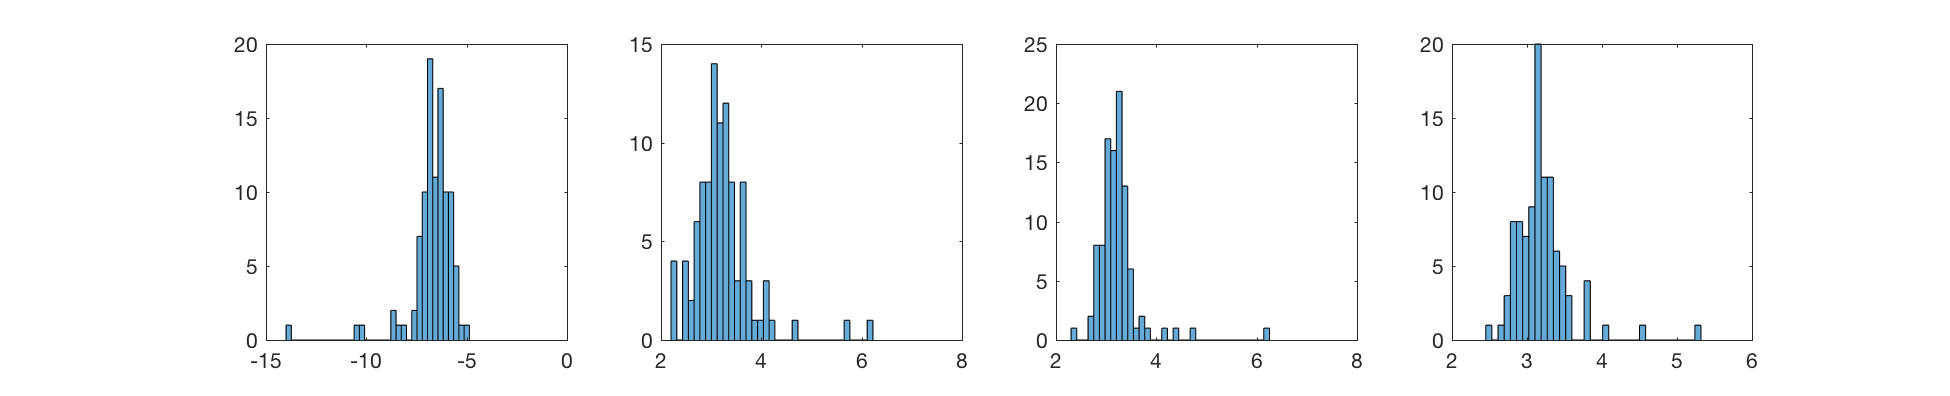
\includegraphics[width=1.2\textwidth]{figures/lte-mean.eps}
    \caption{quasi-posterior mean}
    \label{fig:lte-mean}
\end{figure}

\begin{figure}[hp]
    \centering
    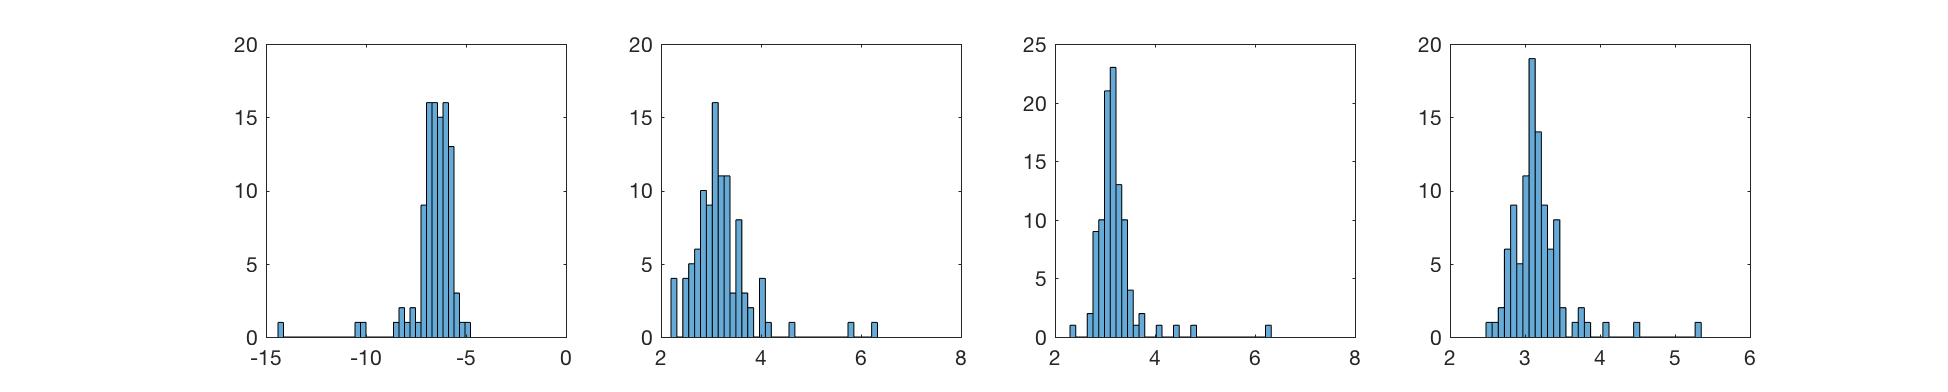
\includegraphics[width=1.2\textwidth]{figures/lte-median.eps}
    \caption{quasi-posterior median}
    \label{fig:lte-median}
\end{figure}

\begin{figure}[hp]
    \centering
    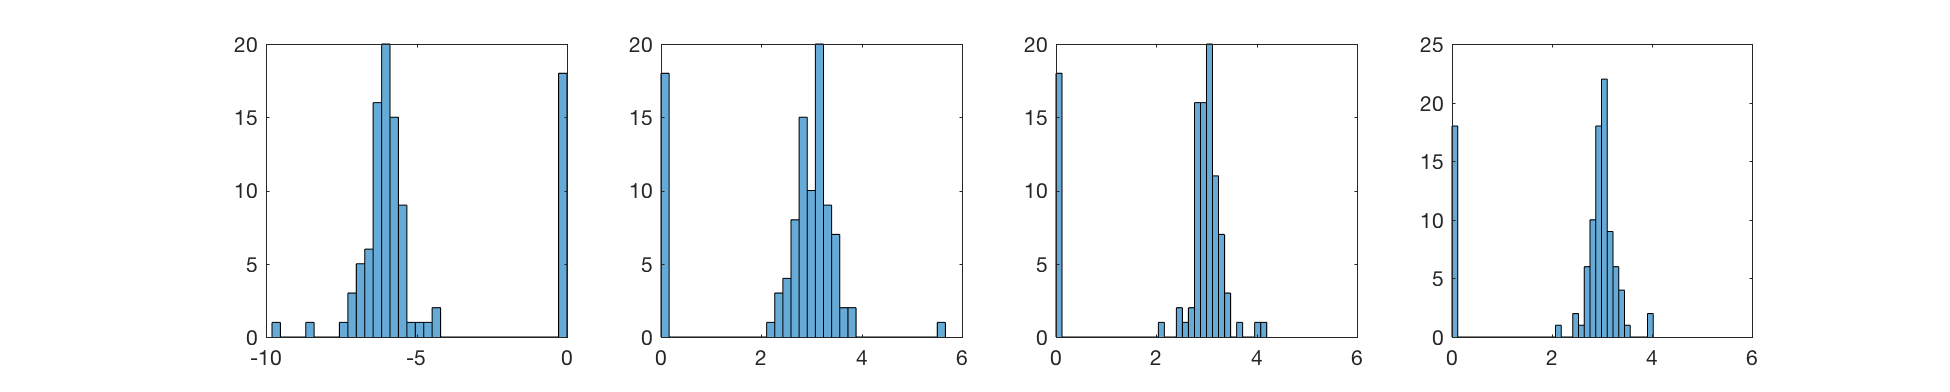
\includegraphics[width=1.2\textwidth]{figures/ilp-allrep.eps}
    \caption{ILP}
    \label{fig:ilp-allrep}
\end{figure}

\begin{figure}[hp]
    \centering
    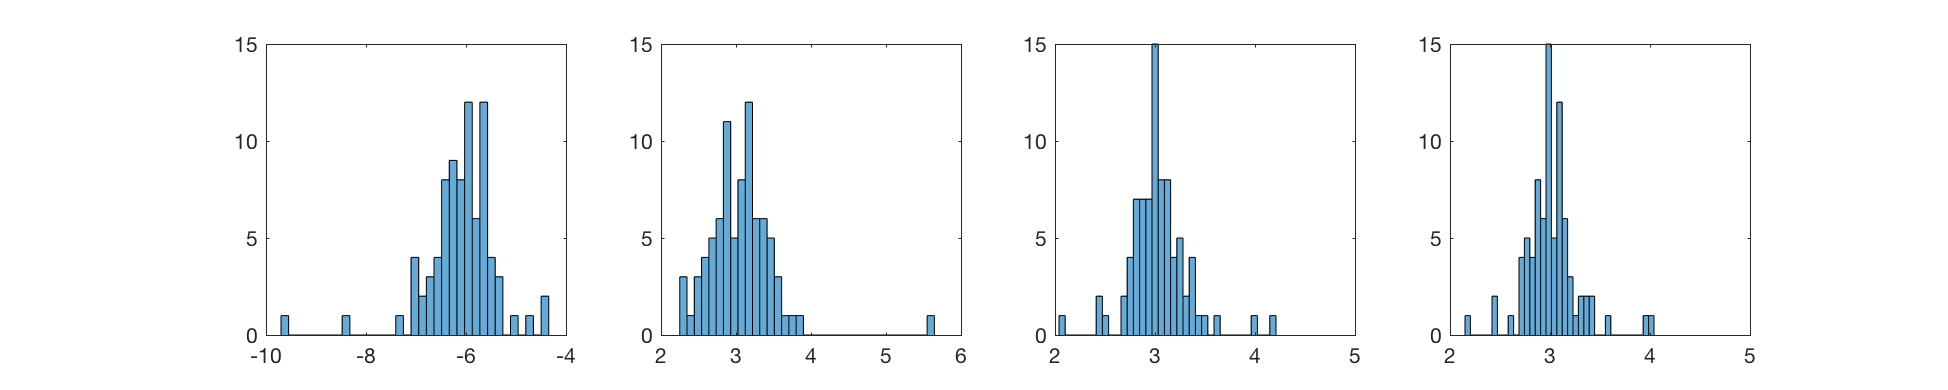
\includegraphics[width=1.2\textwidth]{figures/ilp-exzero.eps}
    \caption{ILP exclude local minimum of zero}
    \label{fig:ilp-exzero}
\end{figure}



\end{document}
